
\documentclass[11pt,a4paper]{article}

\usepackage[T1]{fontenc}
\usepackage{lmodern}
\usepackage[margin=27mm]{geometry}
\usepackage{amsmath,amssymb,mathtools}
\usepackage{enumitem}
\usepackage{microtype}

\setlength{\parindent}{0pt}
\setlength{\parskip}{0.5em}
\setlist[itemize]{leftmargin=2em,itemsep=0.35em}
\setlist[enumerate]{leftmargin=2em,itemsep=0.35em}
\allowdisplaybreaks
\usepackage{tikz}
\usetikzlibrary{arrows.meta}
% Colour Section Titles
\usepackage[dvipsnames]{xcolor}
\usepackage{titlesec}
\usepackage{enumitem}

\definecolor{NitscheBlue}{RGB}{0,136,185}
\definecolor{NitscheGreen}{RGB}{0,135,0}
\definecolor{NitscheMagenta}{RGB}{211,55,213}

% Current heading colour (stored as a name)
\def\currentheadingcolor{Plum}

% Section heading: Plum
\titleformat{\section}
  {\normalfont\Large\bfseries\color{Plum}}
  {\thesection}{1em}{}

% Subsection heading: Orchid
\titleformat{\subsection}
  {\normalfont\large\bfseries\color{Orchid}}
  {\thesubsection}{1em}{}

% For highlightng text
\newcommand{\skyblue}[1]{\textcolor{SkyBlue}{#1}}

\title{\textbf{Summary Notes on Nitsche's Method}}
\author{}
\date{}

\begin{document}
\maketitle

\section{Disclaimer}
These are notes written by chat (edited by me) based off of my handwritten notes. The relevant references are \cite{BenzakenEvansTamstorf2024} and \cite{Shapero2019}.

\section{Shapero's Note \cite{Shapero2019}}

\begin{itemize}
    \item Considers Poisson's problem with Dirichlet conditions.

    \item Introduces Nitsche's method as a way to alter the variational principle to impose boundary conditions. This is especially helpful for problems which do not have an obvious way to impose essential boundary conditions.
\end{itemize}

\subsection{Penalty Method}

\begin{itemize}
    \item View Dirichlet boundary conditions as a constraint for an energy minimisation problem.

    \item Then use a penalty method.

    \item As $\gamma\to\infty$, you recover the original problem.

    \item The issue is ill-conditioning as $\gamma\to\infty$, and that $\gamma\sim h^{-1}$ reduces $O(h^p)$ accuracy to $O(h^{p/2})$ accuracy.
\end{itemize}

\subsection{Lagrange Multiplier Method}

\begin{itemize}
    \item Instead, introduce a Lagrange multiplier for the constraint and solve the system obtained from stationarity of the Lagrangian.

    \item But now we have introduced a saddle-point problem for which we need to worry about stability.

    \item However, from this approach, we learn that the Lagrange multiplier is related to the boundary flux:
    \[
        \lambda=-k\frac{\partial u}{\partial n},
    \]
    where we minimise
    \[
        J(u)=\int_\Omega\left(\frac12 k|\nabla u|^2-fu\right)\,dx,
        \qquad\text{subject to }u|_{\partial\Omega}=g.
    \]
\end{itemize}

\subsection{Augmented Lagrangian Method}

\begin{itemize}
    \item Combines the penalty and Lagrange multiplier methods. This eliminates the need for $\gamma\to\infty$, and we avoid the discretisation issues of the Lagrange multiplier method.

    \item We get a positive-definite problem for the solution $u$, and we get exact enforcement of $u=g$ without taking $\gamma\to\infty$.
\end{itemize}

\subsection{Nitsche's Method}

\begin{itemize}
    \item Finally, we substitute $\lambda=-k\frac{\partial u}{\partial n}$ (learned from the Lagrange multiplier approach) into the augmented Lagrangian method.

    \item He uses Young's $\varepsilon$-inequality (Peter--Paul inequality) and an inverse inequality to find a condition on the penalty parameter $\gamma$ so that the exact solution is a minimiser of the Nitsche formulation (consistency).
\end{itemize}

\newpage

\section{Benazaken, Evans, Tamstorf (Disney Animators) Paper \cite{BenzakenEvansTamstorf2024}}

\subsection{Introduction}

\begin{itemize}
    \item Nitsche's method is used to weakly enforce boundary conditions. It results in a formulation that is consistent, stable, and has optimal convergence rates after discretisation.

    \item It avoids the issues of both the penalty and Lagrange multiplier methods. It does not result in a saddle-point problem, and it can achieve accurate results for moderately sized penalty parameters (leading to relatively well-conditioned symmetric positive-definite (SPD) linear systems after discretising self-adjoint elliptic PDEs).

    \item Nitsche's method adds a penalty term to enforce Dirichlet boundary conditions, consistency terms to restore the variational consistency lost when we choose not to strongly enforce the boundary conditions, and symmetry terms to make the resulting bilinear form symmetric.
\end{itemize}

\subsection{The Abstract Formulation}

\begin{itemize}
    \item Let $V$ and $Q$ be Hilbert spaces (with their usual inner products and induced norms). Let $V^*$ and $Q^*$ be their duals, respectively. Use ${}_{V^*}\langle\cdot,\cdot\rangle_V$ and ${}_{Q^*}\langle\cdot,\cdot\rangle_Q$ for their duality pairings, respectively.

    \item Let $T:V\to Q$ be the bounded, surjective trace operator.

    \item Let
    \[
        V_g=\{v\in V:T v=g\},\qquad g\in Q.
    \]

    \item Let $a:V\times V\to\mathbb R$ be a bounded, symmetric, positive-semidefinite bilinear form that satisfies
    \[
        a(v,v)\ge C\|v\|_V^2\qquad\forall v\in V_0,
    \]
    for some constant $C\in\mathbb R_+$.

    \item The minimisation problem of interest is:
    \[
        \boxed{\begin{gathered}
            \text{Given }f\in V^*\text{ and }g\in Q,\text{ find }u\in V_g
            \text{ that minimises}\\
            E_{\mathrm{total}}(u)=E_{\mathrm{int}}(u)+E_{\mathrm{ext}}(u),\\
            E_{\mathrm{int}}(u)=\frac12 a(u,u),\qquad
            E_{\mathrm{ext}}(u)=-{}_{V^*}\langle f,u\rangle_V.
        \end{gathered}}
    \]

    \item Fun fact: The negative sign in $-{}_{V^*}\langle f,v\rangle_V$ signifies the forces that induce the displacement field, which do work on the system.

    \item The corresponding variational problem is to
    \[
        \boxed{\text{Find }u\in V_g\text{ such that }
        a(u,\delta u)={}_{V^*}\langle f,\delta u\rangle_V
        \quad\forall\delta u\in V_0.}
    \]

    \item As usual, we approximate $u$ with $u_h$ by restricting to
    \[
        V_{g,h}=V_h\cap V_g,\qquad V_h\subset V.
    \]

    \item For Nitsche's method to be successful, we must satisfy two assumptions:
\end{itemize}

\subsubsection*{1. Generalised Green's Identity $\longrightarrow$ Consistency}

\begin{enumerate}[label=(\alph*)]
    \item There is a dense subset $\widetilde V\subset V$ and linear maps
    \[
        L:\widetilde V\to V^*,\qquad B:\widetilde V\to Q^*,
    \]
    such that the following generalised Green's identity holds:
    \[
        a(w,v)={}_{V^*}\langle Lw,v\rangle_V
                 +{}_{Q^*}\langle Bw,Tv\rangle_Q.
    \]

    \item The exact solution $u$ satisfies $Lu=f$ whenever $u\in\widetilde V$.
\end{enumerate}

\textbf{Explanation}

\begin{itemize}
    \item (a) asks for integration by parts to exist. $\widetilde V$ is the extra regularity needed for this to hold.

    \item (b) asks for consistency: $a(u-u_h,v_h)=0$ when we have enough regularity. In particular, we ask what boundary terms we need so that a sufficiently regular exact solution also satisfies Nitsche's formulation? 

    \item Typically, $L$ encodes the differential operator of the strong problem, with boundary conditions encoded by $B$.
\end{itemize}

\subsubsection*{2. Generalised Trace and Cauchy--Schwarz $\longrightarrow$ Well-posedness and quasi-optimality.}

We assume that there are densely defined, positive, self-adjoint linear maps
\[
    \eta:\operatorname{dom}(\eta)\subseteq Q^*\to Q,
    \qquad
    \varepsilon:\operatorname{dom}(\varepsilon)\subseteq Q^*\to Q,
\]
with $\varepsilon$ invertible, such that:

\begin{enumerate}[label=(\alph*)]
    \item The domain of definition of $B:\widetilde V\to Q^*$ can be extended to $\widetilde V+V_h$, and
    \[
        \{Bv:v\in\widetilde V+V_h\}\subseteq\operatorname{dom}(\eta).
    \]

    \item The generalised trace inequality
    \[
        {}_{Q^*}\langle Bv_h,\eta Bv_h\rangle_Q
        \le a(v_h,v_h)
    \]
    holds for all $v_h\in V_h$.

    \item The generalised Cauchy--Schwarz inequality
    \[
        \left|{}_{Q^*}\langle Bv,Tw\rangle_Q\right|
        \le \frac1\gamma
        \left({}_{Q^*}\langle Bv,\eta Bv\rangle_Q\right)^{1/2}
        \left({}_{Q^*}\langle\varepsilon^{-1}Tw,Tw\rangle_Q\right)^{1/2}
    \]
    holds for all $v,w\in\widetilde V+V_h$, where $\gamma\in(1,\infty)$.
\end{enumerate}

\textbf{Explanation}

\begin{itemize}
    \item $\eta$ and $\varepsilon$ can almost be thought of as Riesz operators. They are necessary to form a duality pairing between $Bv_h$ and itself, and $Tw$ and itself:
    \[
        (Bv_h,Bv_h)_{Q^*}=\|Bv_h\|_{Q^*}^2
        \qquad\text{vs.}\qquad
        {}_{Q^*}\langle Bv_h,\eta Bv_h\rangle_Q
        \quad\text{(duality pairing)}.
    \]

    \item Notice that $V_h$ need not be a subset of $\widetilde V$, but we need to apply $B$ to elements in $V_h$. Thus, we extend the domain of $B$ to $\widetilde V+V_h$.

\end{itemize}

\subsection{Nitsche's Method for an Abstract Variational Problem}


Given $f\in V^*$ and $g\in Q$, find $u_h\in V_h$ such that
\begin{align*}
a_h(u_h,\delta u_h)
={}&{}_{V^*}\langle f,\delta u_h\rangle_V\\[0.75em]
&\quad
\textcolor{NitscheGreen}{
\underbrace{
-{}_{Q^*}\langle B\delta u_h,g\rangle_Q
}_{\text{Symmetry Term}}}\\[0.5em]
&\quad
\textcolor{NitscheMagenta}{
\underbrace{
+{}_{Q^*}\langle\varepsilon^{-1}T\delta u_h,g\rangle_Q
}_{\text{Penalty Term}}}
\end{align*}
for every $\delta u_h\in V_h$, where
$a_h:(\widetilde V+V_h)\times(\widetilde V+V_h)\to\mathbb R$
is the bilinear form defined by
\begin{align*}
a_h(w,v)
={}&a(w,v)\\[0.5em]
&\quad
\textcolor{NitscheBlue}{
\underbrace{
-{}_{Q^*}\langle Bw,Tv\rangle_Q
}_{\text{Consistency Term}}}\\[1.5em]
&\quad
\textcolor{NitscheGreen}{
\underbrace{
-{}_{Q^*}\langle Bv,Tw\rangle_Q
}_{\text{Symmetry Term}}}\\[1.5em]
&\quad
\textcolor{NitscheMagenta}{
\underbrace{
+{}_{Q^*}\langle\varepsilon^{-1}Tv,Tw\rangle_Q
}_{\text{Penalty Term}}},
\end{align*}
for all $w,v\in\widetilde V+V_h$.

\newpage

\textbf{Notes}

\begin{itemize}
    \item This is a well-posed problem (unique, stable solution) that is consistent (the exact solution of the original strong problem satisfies it, giving Galerkin orthogonality). It is also quasi-optimal (we can apply C\'ea's lemma).

    \item Assumption 1 grants consistency; Assumption 2 grants continuity and coercivity.

    \item Consistency ensures that even though the additional terms change the discrete problem, they preserve the exact solution of the original variational problem. Combined with the trace and Cauchy--Schwarz inequality, we get the needed well-posedness and quasi-optimality.

    \item The process:
    % \[
    % \text{Assumption 1}\Longrightarrow\text{Consistency}
    % \Longrightarrow\text{Galerkin orthogonality}.
    % \]
    % \[
    % \begin{gathered}
    % \text{Assumption 2}\Longrightarrow\text{Coercivity and continuity}\\
    % \Longrightarrow\text{Well-posedness and quasi-optimality}
    % \Longrightarrow\text{Convergence}.
    % \end{gathered}
    % \]

    
\begin{center}
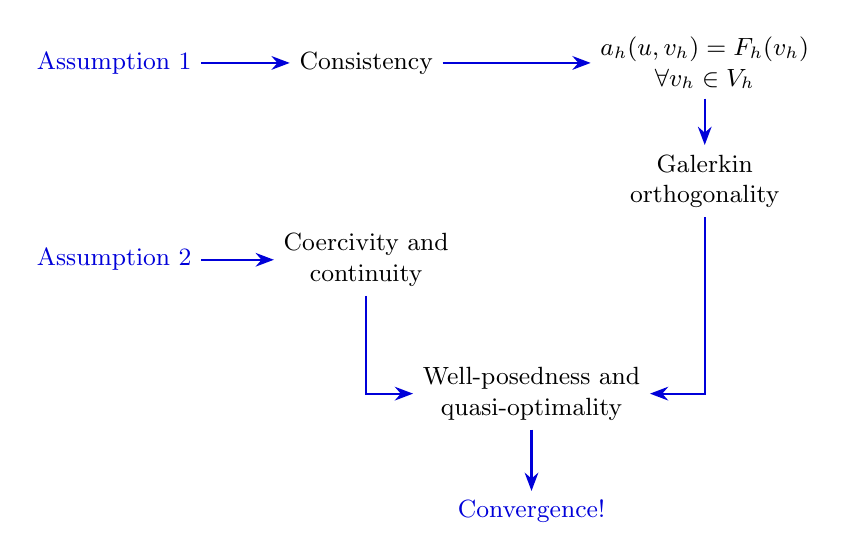
\begin{tikzpicture}[
    >=Stealth,
    every node/.style={align=center, font=\small},
    arr/.style={->, thick, blue!85!black}
]

% Assumption 1: Consistency
\node[text=blue!85!black] (a1) at (0,3)
    {Assumption 1};
\node (cons) at (3.2,3)
    {Consistency};
\node (exact) at (7.5,3)
    {$a_h(u,v_h)=F_h(v_h)$\\
     $\forall v_h\in V_h$};
\node (orth) at (7.5,1.5)
    {Galerkin\\orthogonality};

% Assumption 2: Stability
\node[text=blue!85!black] (a2) at (0,0.5)
    {Assumption 2};
\node (stab) at (3.2,0.5)
    {Coercivity and\\continuity};

% Conclusions
\node (well) at (5.3,-1.2)
    {Well-posedness and\\quasi-optimality};
\node[text=blue!85!black] (conv) at (5.3,-2.7)
    {Convergence!};

% Arrows
\draw[arr] (a1) -- (cons);
\draw[arr] (cons) -- (exact);
\draw[arr] (exact) -- (orth);

\draw[arr] (a2) -- (stab);
\draw[arr] (stab.south) |- (well.west);
\draw[arr] (orth.south) |- (well.east);

\draw[arr] (well) -- (conv);

\end{tikzpicture}
\end{center}

\end{itemize}

\newpage

\section*{For the Biharmonic Problem}

\begin{itemize}
    \item The problem considered is
    \[
    \begin{cases}
       \Delta^2u=F &\text{in }\Omega,\\
       u=g &\text{on }\Gamma_{D_1},\\
       \partial_n u=h &\text{on }\Gamma_{D_2},\\
       \partial_n(\Delta u)=p &\text{on }\Gamma_{N_1},\\
       \Delta u=q &\text{on }\Gamma_{N_2}.
    \end{cases}
    \]

    \item Following the abstract methodology, Nitsche's method is as follows.
\end{itemize}

\subsection{Nitsche's Method for the Biharmonic Problem}

Given $f^B\in(V^B)^*$ and $(g,h)\in Q^B$, find $u_h\in V_h^B$ such that
\begin{align*}
a_h^B(u_h,\delta u_h)
={}&
\underbrace{
\begin{aligned}
&\int_\Omega f\cdot\delta u_h\,d\Omega
-\int_{\Gamma_{N_1}}p\cdot\delta u_h\,d\Gamma\\
&+\int_{\Gamma_{N_2}}q\cdot[(\nabla\delta u_h)\cdot\mathbf n]\,d\Gamma
\end{aligned}
}_{\langle f^B,\delta u_h\rangle}\\[1.5em]
&\quad
\textcolor{NitscheGreen}{
\underbrace{
\begin{aligned}
&+\sum_{E_1\in\mathcal E_{D_1}}\int_{E_1}
[(\nabla\Delta\delta u_h)\cdot\mathbf n]\cdot g\,d\Gamma\\
&-\sum_{E_2\in\mathcal E_{D_2}}\int_{E_2}
(\Delta\delta u_h)\cdot h\,d\Gamma
\end{aligned}
}_{\text{Symmetry Terms}}}\\[1.5em]
&\quad
\textcolor{NitscheMagenta}{
\underbrace{
\begin{aligned}
&+\sum_{E_1\in\mathcal E_{D_1}}\int_{E_1}
\frac{C_{\mathrm{pen},1}^B}{h_{E_1}^3}
\delta u_h\cdot g\,d\Gamma\\
&+\sum_{E_2\in\mathcal E_{D_2}}\int_{E_2}
\frac{C_{\mathrm{pen},2}^B}{h_{E_2}}
[(\nabla\delta u_h)\cdot\mathbf n]\cdot h\,d\Gamma
\end{aligned}
}_{\text{Penalty Terms}}}
\end{align*}
for every $\delta u_h\in V_h^B$, where
$a_h^B:(\widetilde V^B+V_h^B)\times(\widetilde V^B+V_h^B)\to\mathbb R$
is the bilinear form defined by
\begin{align*}
a_h^B(w_h,v_h)
={}&
\underbrace{
\int_\Omega(\Delta w_h)\cdot(\Delta v_h)\,d\Omega
}_{a^B(w_h,v_h)}\\[1.5em]
&\quad
\textcolor{NitscheBlue}{
\underbrace{
\begin{aligned}
&+\sum_{E_1\in\mathcal E_{D_1}}\int_{E_1}
[(\nabla\Delta w_h)\cdot\mathbf n]\cdot v_h\,d\Gamma\\
&-\sum_{E_2\in\mathcal E_{D_2}}\int_{E_2}
(\Delta w_h)\cdot[(\nabla v_h)\cdot\mathbf n]\,d\Gamma
\end{aligned}
}_{\text{Consistency Terms}}}\\[1.5em]
&\quad
\textcolor{NitscheGreen}{
\underbrace{
\begin{aligned}
&+\sum_{E_1\in\mathcal E_{D_1}}\int_{E_1}
[(\nabla\Delta v_h)\cdot\mathbf n]\cdot w_h\,d\Gamma\\
&-\sum_{E_2\in\mathcal E_{D_2}}\int_{E_2}
(\Delta v_h)\cdot[(\nabla w_h)\cdot\mathbf n]\,d\Gamma
\end{aligned}
}_{\text{Symmetry Terms}}}\\[1.5em]
&\quad
\textcolor{NitscheMagenta}{
\underbrace{
\begin{aligned}
&+\sum_{E_1\in\mathcal E_{D_1}}\int_{E_1}
\frac{C_{\mathrm{pen},1}^B}{h_{E_1}^3}
w_h\cdot v_h\,d\Gamma\\
&+\sum_{E_2\in\mathcal E_{D_2}}\int_{E_2}
\frac{C_{\mathrm{pen},2}^B}{h_{E_2}}
[(\nabla v_h)\cdot\mathbf n]
\cdot[(\nabla w_h)\cdot\mathbf n]\,d\Gamma
\end{aligned}
}_{\text{Penalty Terms}}},
\end{align*}
for all $w_h,v_h\in\widetilde V^B+V_h^B$.

In satisfying the two assumptions, this formulation is well-posed and quasi-optimal.

\subsection{Notes on Derivation and Proofs}

\begin{itemize}
    \item The choice of penalty parameter follows from a generalised eigenproblem used to prove/derive the needed trace inequalities. I do not think these are solved much in practice.

    \item For clamped conditions, $\Gamma_{D_1}=\Gamma_{D_2}=\partial\Omega$ and $\Gamma_{N_1}=\Gamma_{N_2}=\varnothing$.

    \item For homogeneous clamped conditions, $g=h=0$, so the right-hand side becomes
    \[
       \int_\Omega F\,\delta u_h\,dx.
    \]
\end{itemize}


\bibliography{Nitsche}
\bibliographystyle{plain}
\end{document}
